\section{Implementation and Runtime}
In this section we discuss our extensions to 
the MapReduce programming model and shows the major changes to runtime to 
support \myds
to support pipelining between Map and Reduce (Section 3.2). 
We describe how our design supports
piplelining (Section 3.3), and discuss the buffer design (Section 3.4). 
Our focus here is on Producer-Consumer model; 
We defer performance results to Section 5.



\subsection{Execution flow}
\begin{figure}[!h!t]  
    \centering
    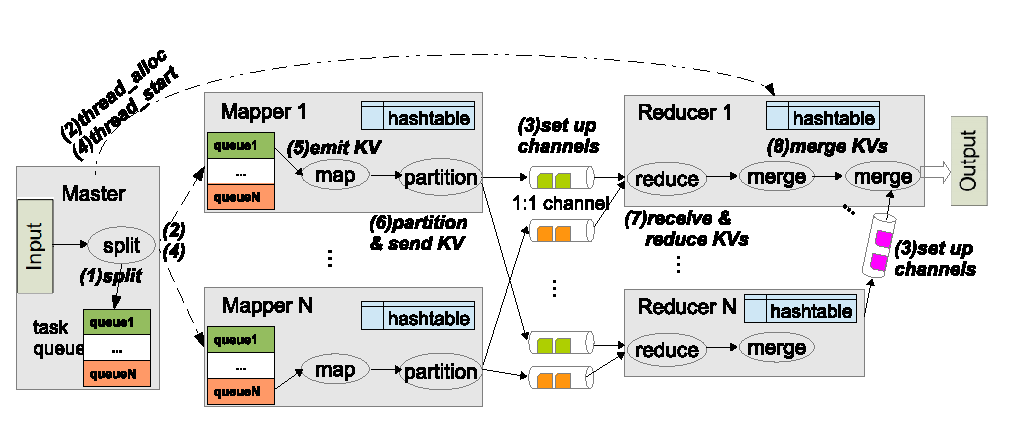
\includegraphics[width=0.45\textwidth]{eps/dmr.eps}
    \caption{Deterministic execution flow of DMR}
    \label{fig:dmr:flow}
\end{figure}

%不同与Phoenix,DMR将任务队列静态的划分给每个map worker,这样做的好处是,可以避免多个map worker对对任务队列操作从而产生锁的开销。
DMR’s implementation of MapReduce closely resembles Phoenix’s. 
There is a single master managing a number of slaves. 
The input file is split into even-sized chunks replicated. 
DMR divides each MapReduce job into a set of tasks. 

Each chunk of input is first processed by a map task, 
which outputs a list of key-value pairs generated 
by a user-defined map function. 
Map outputs are split into buckets based on key. 
When all maps have finished, reduce tasks
apply a reduce function to the list of map outputs with
each key. Figure\ref{fig:dmr:flow} illustrates a MapReduce computation.

For a reduce task, the execution is divided into
three phases:
\begin{itemize}
  \item The copy phase, when the task fetches map outputs.
  \item The sort phase, when map outputs are sorted by key.
  \item The reduce phase, when a user-defined function is
applied to the list of map outputs with each key.
\end{itemize}




Figure\ref{fig:dmr:flow} shows the data flow for 
\myds runtime system, 
including three main phases: map, reduce, and merge.
There are two key points for DMR runtime comparied to Phoenix.
First, it schedules map tasks in round-robin manner+
and add a partition operation for reduce tasks 
to ensrue deterministic shceduling.
Second, it broke barrier between map and reduce phase,
which is neccessary to Phoenix,
then reducers can start work before all of mappers finished.

The map phase reads the task’s split from task queue,
parses it into key-value pairs, and applies
the map function to each record.
Intermediate keys are assigned
to reducers by applying a partitioning function
A spill of the in-memory buffer involves first sorting
the records in the buffer by partition number and then by
key.

After receiving its partition from all map outputs, the
reduce task enters the sort phase. The map output for
each partition is already sorted by the reduce key. The
reduce task merges these runs together to produce a sin-
gle run that is sorted by key. The task then enters the
reduce phase, in which it invokes the user-defined reduce
function for each distinct key in sorted order, passing it
the associated list of values.

We addressed these issues by buffering the mapper output until
it reaches a certain record threshold.
When the record threshold isreached, 
the mapper sends the output to a reducer. 
Next, Reducer receives its partition from all map, 
and enters the sort phase.
%将之前对combiner和merge阶段的特征进行简单的总结
{\bf Combiner.}
In order to maximally reduce memory pressure due to intermediate key-value
storage.%通道的数据流通量(map和reduce见传递的数据量)
%做法,开销,优势,我们的特点,可以在reduce阶段进行combiner
The imbalance of tasks can be solved by dynamic scheduling in the Map phase. 
%%事实上,为了防止出现数据倾斜的问题,即map阶段的很多key都发送到一个reduce,导致某个reduce有过多的动态内存分配,甚至可能出现内存不够的情况,我们可以对reduce的数据做局部的combiner
%However, in the Reduce phase, 
%as all values for the same key must be in one reduce task, 
%it is not always feasible to generate a large number reduce tasks for
%%dynamic scheduling.

{\bf merge.}
Each Reduce generates a set of output key/value
pairs, and the library’s Merge phase sorts them by key to
produce the final output. 
%做法,作用,我们的优化,不需要进行reduce和merge的阶段,应当尽量避免,以降低时间的开销

\subsection{Pipelined execution}
Pipelined map and reduce has been adopted 
in the MapReduce framework for distributed computing\cite{Condie2010MapReduce,}. 
Condie et al. show that since the intermediate data is delivered to
downstream operators more promptly, 
it is able to improve resource utilization.

%In general MapReduce programming model, 
While in Phoenix, (To avoid mulit map and reduce contention the same area, )
there is a strict barrier between the Map and Reduce phases: 
the workers in one phase can only be started 
until all workers in the previous phase has been finished. 
Hence, the execution time of a job is determined by the
slowest worker in each phase. 
A downstream dataflow element can begin consuming data
before a producer element has finished execution, which can
increase opportunities for parallelism, improve utilization,
and reduce response time.
On the other hand, MapReduce workloads
are an ideal candidate for pipelining as the user-defined
map functions are usually computation-intensive, while the
reduce phase to construct the global container is memory
intensive\cite{talbot2011phoenix++}.
Overlapping the
computation-intensive and memory-intensive workloads 
can effective improve the overall hardware resource utilization.

%我们设计了一个生产者和消费者模型,用于map和reduc阶段的流水并行,有两个重要的数据结构:map worker的buffer池,reducer worker的全局buffer。每个map worker拥有一个私有的buffer池,当key-value产生后,通过partition函数插入到对应的buffer中。其中每个buffer对应一个reduce worker,reduce worker轮循的从各个map的buffer池中取key-value,并调用reduce函数进行计算;每个reduce拥有一个私有的全局buffer,用于存放reduce处理后得到的全局结果。
We design a producer-consumer model to pipeline the
map and reduce phases.
There are two major data structures,
which are local buffers pool for map worker and 
a global buffer for reduce worker.
Specifically, 
each map worker has a local buffers pool and 
each buffer for a corresponding reduce worker.
Partition function will be used to push key-value into a corresponding
buffer.
When the buffer threshold isreached,
the corresponding reduce worker can read record in the buffer.
One reduce worker will get key-value from each map by Round-Robin and 
merge the key-value pairs to the global buffer.


%如同Phoenix, 默认情况下,buffer使用hash table来实现,事实上,在我们的模型中,使用array来实现具有更好的性能。下面的章节会详细解释原因。
Defaultly, the buffer is a hash table as Phoenix.
While this technique is more effective for the array buffer
container than the hash buffer. 
We will explain the advantage of array buffer in section 3.2.1.
MRPhi\cite{lu2013mrphi} is also use producer-consumer model to 
pipeline the map and reduce phases. 
There are partitions queues for each reduce worker.
While we don't use queues, mapping will be used in DMR(section 3.2.2).

%(The motivation is that the map function defined by users
%usually performs heavy computation. But the reduce phase
%contains many memory accesses in which the major work is to
%construct the global container. 
% )

\input buffer

\subsubsection{Producer-Consumer model}
The pipelined map and reduce are implemented using a
producer-consumer model. 
The map and reduce workers are the producers and consumers, respectively.
Specially, the map worker generate key-value and 
put it into the buffer.
At the same time, 
the reduce worker is consuming the key-value.
%由于map和reduce worker共享这个buffer,因此最关键的问题是如何同步
As the buffer is a shared region of memory in tradition,
either a map worker or a single reduce worker,
can access the structure at any given time.
%使用queue
In fact, producer-consumer model implementations
often use a shared queue.

MRphi\cite{lu2013mrphi}design a producer-consumer model 
to pipeline the map and reduce phases. 
There are three major data structures, 
which are local hash tables, a global hash table, 
and partition queues. 
Specifically, each map worker has a local hash table. 
When a local hash table is full,
key-value pairs stored in this table are partitioned and
pushed into corresponding queues. 
Meanwhile, one reduce
worker works on one queue to merge the key-value pairs to
the final global hash table.

There three differences DMR and MRphi:
(1) when the map local hash table is full,
key-value pairs stored in this table are partitioned and
pushed into corresponding queues.
%hash table 数据分布不均匀,如果只是简单的做一个 partition,可能导致有些 reduce task很小,甚至为空。而每次的将 reduce task 加入到 queue 都需要同步的开销
(2) when map worker insert reduce taskes to the queue of reduce,
the map worker is stoped to wait.
%map worker 将 reduce task 插入到 queue 这个过程,需要停下来等待,无形中延迟了 map 的执行时间
(3)%多个 map worker 会同时对 reduce worker 的 queue 进行操作,需要相应的同步手段,由此会产生等待开销。核数越多,开销会越明显。
As the queue of reduce worker will be operation by multi map worker,

t is important for databases and large web and proxy servers to map files into memory instead of having a buffer and reading the file contents into the buffer. If you map the file into memory directly, the operating system has more memory left for I/O buffering.


Figure\ref{fig:dmr:spmc}
\begin{figure}[!h!t]
    \centering
    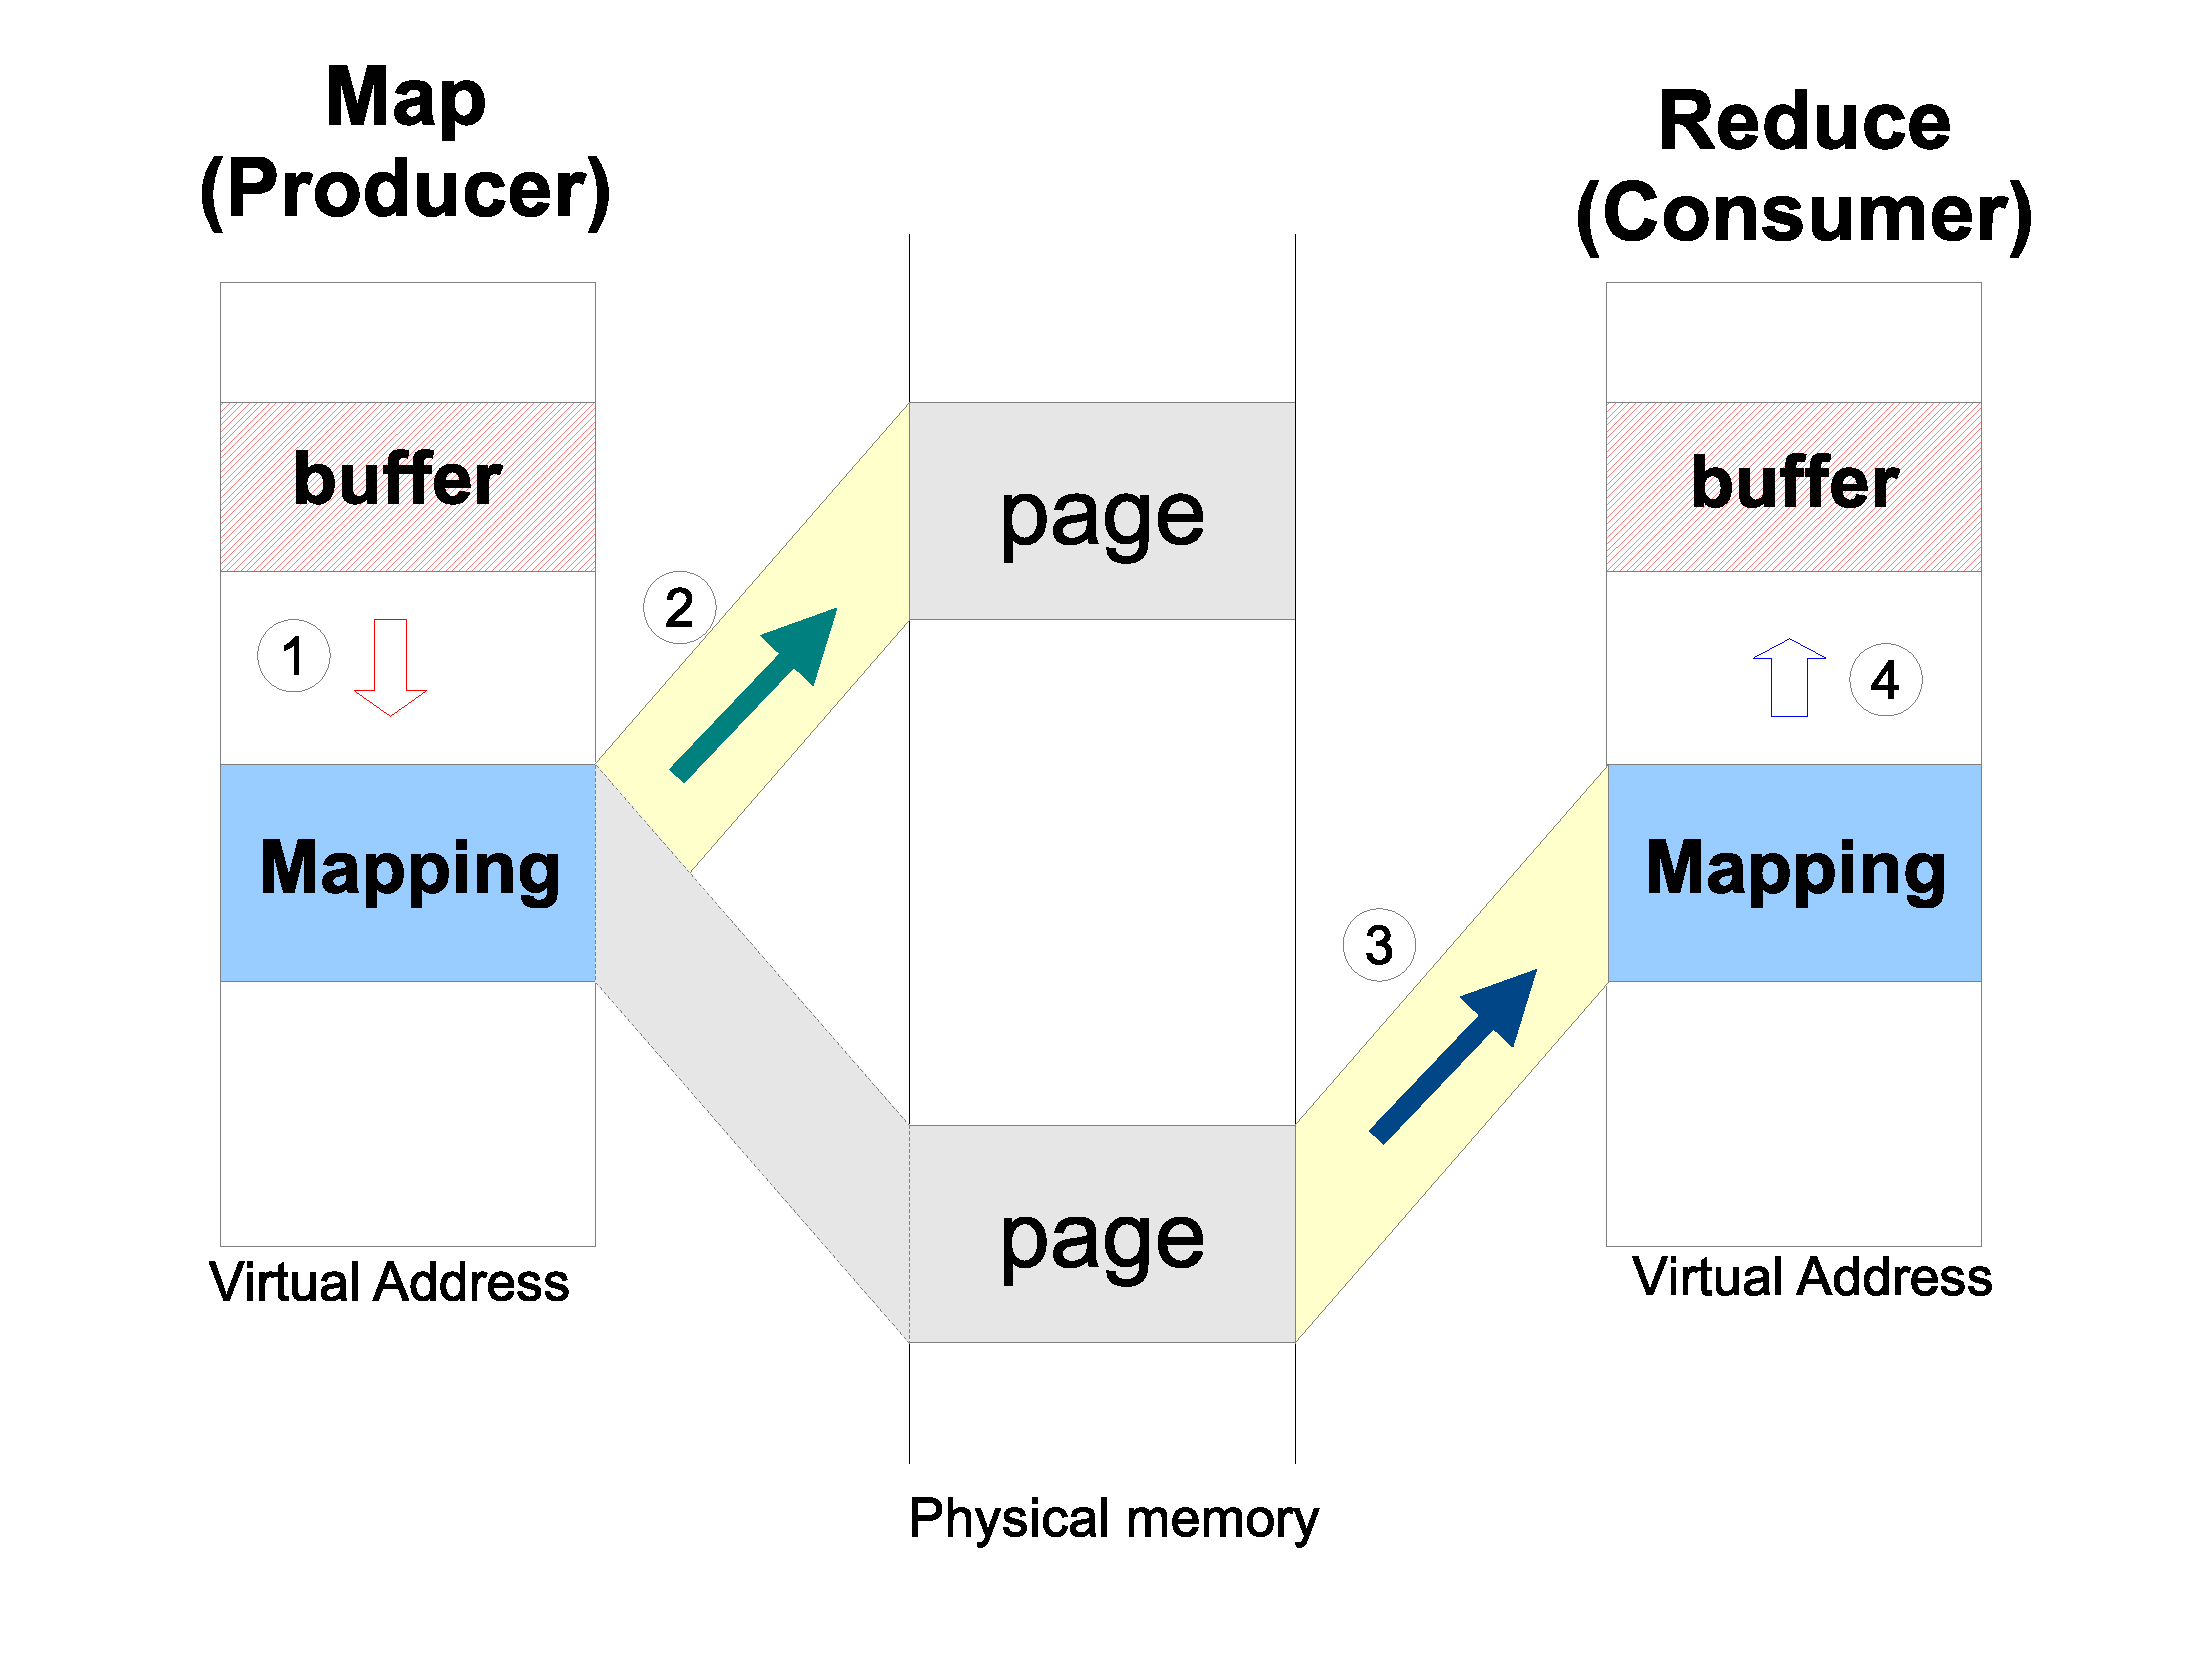
\includegraphics[width=0.45\textwidth]{eps/dmr_pc_model.eps}
    \caption{producer-consumer model}
    \label{fig:dmr:spmc}
\end{figure}
%SPMC的快速
{\color{gray}
In the shared-memory model, a region of memory that is shared
by cooperating processes is established. 
Processes can then exchange information 
by reading and writing data to the shared region.
Shared memory can be faster.
since in shared-memory systems, system calls are required only to establish shared-memory regions. 
Once shared memory is established, all accesses are treated
as routine memory accesses, and no assistance from the kernel is required.
}
%SPMC区域的建立
Interprocess communication using shared memory requires communicating
processes to establish a region of shared memory. Typically, a shared-memory
region resides in the address space of the process creating the shared-memory
segment. Other processes that wish to communicate using this shared-memory
segment must attach it to their address space. 

%SPMC区域的使用,对应buffer
To allow producer and consumer processes to run concurrently, we must have
available a buffer of items that can be filled by the producer and emptied by
the consumer. This buffer will reside in a region of memory that is shared by
the producer and consumer processes.(http://bulk.fefe.de/scalability/)



\subsection{Separate Address Space}
%先详细分析Phoenix使用线程存在的问题,然后我们采用进程地址空间隔离会有哪些好处
%虽然MRPhi中也是使用producer-consumer model,DMR不同之处在于,(1)它不需要显示的管理map和reduce间的队列,简单;(2)
In addition to global locks like the ones discussed earlier, 
data structure private locks can also be a problem 
if the data structure is shared by multiple threads. 
A standard example here are the mm\_sem read-write semaphore 
that protects the list of mappings in a process and 
the pagetable\_lock that protects the pagetable state of a process. 
These locks are local to a process’ address space. 
However when the process is using multiple threads 
then these threads will be able to access the address space in parallel,
which can cause contention on these locks. 
A classical example here is 
the initialization of a large multi-threaded computing job 
that causes a lot of parallel page-faults. 
These page-faults will all run into contention on the mm\_sem semaphores. Semaphores are sleeping locks 
and may run into convoying problems 
where waiting threads may 
get stuck at the end of the wait queue for a long time.\cite{Andi2009lmulticore}

Unfortunately these programs are often written to start as many threads as the system has CPUs, 
but when the system is larger than their scalability limit adding more threads might actually scale negatively.
The first measure is to limit them to the maximum number of threads that they can successfully scale to.
This of course leaves some of the CPUs idle. 




There is a sense in the community that traditional kernel
designs won’t scale well on multicore processors: that
applications will spend an increasing fraction of their time
in the kernel as the number of cores increases.

To understand the Linux scalability
behavior, we analyze the related implementation of Linux
kernel and exploit performance tools to identify scalability
bottlenecks.


As indicated by this figure, the time of completing
a workload for one core increases when there are more
cores in the system. The trend of this curve suggests that
the parallel scalability of forkbench is poor.

In order to understand the scalability behavior, 
Perf\cite{} is exploited to collect execution time information
on the function basis. 
Experimental results on 32 cores
show that \_\_ticket\_spin\_lock and 
default\_send\_IPI\_mask\_sequence\_phys are two functions 
which have largest execution time with 71.25\% and 10.20\% respectively. 

Performance data reveal that two functions vma link() and
unlink file vma() have the largest execution time (46.02%
and 49.97\%) and lock contention. Call-graph information
and source code analysis show that the two functions are
called when adding a virtual memory address range into the
process address space or deleting a virtual memory address range. 
When multiple slave processes call mmap() or unmap() concurrently, the 
memory mapped file address range should be added into or 
deleted from each slave process address space. However, 
the same spin lock protecting the memory mapped file 
address range should be held or released. Thus, spin lock 
contention degrades the parallel scalability performance of 
the benchmark. 



The difference between processes and threads under Linux 2.4 is that threads share more parts of their state (address space, file handles etc) than processes, 

